\documentclass[a4paper, 12pt]{article}

%%% SST LAB PROTOCOLL PREAMBLE
%%% 2019
%%%%%%%%%%%%%%%%%%%%%%%%%%%%%%%


%%% PACKAGES
%%%%%%%%%%%%%%%%%%%%%%%%%%%

\usepackage[ngerman]{babel}

\usepackage[utf8]{inputenc}
\usepackage{amsmath}
\usepackage{pgfplots}
\usepackage{tikz}
\usepackage[many]{tcolorbox}
\usepackage{graphicx}
\graphicspath{ {./graphics/} }
\usepackage{pdfpages}
\usepackage{dashrule}
\usepackage{float}
\usepackage{siunitx}
\usepackage{booktabs}
\usepackage[version=4]{mhchem}

%%% DOCUMENT GEOMETRY
%%%%%%%%%%%%%%%%%%%%%%%%%%%

\usepackage{geometry}
\geometry{
 a4paper,
 total={0.6180339887498948\paperwidth,0.6180339887498948\paperheight},
 top = 0.1458980337503154\paperheight,
 bottom = 0.1458980337503154\paperheight
 }
\setlength{\jot}{0.013155617496424828\paperheight}
\linespread{1.1458980337503154}

\setlength{\parskip}{0.013155617496424828\paperheight} % paragraph spacing


%%% COLORS
%%%%%%%%%%%%%%%%%%%%%%%%%%%

\definecolor{red1}{HTML}{f38181}
\definecolor{yellow1}{HTML}{fce38a}
\definecolor{green1}{HTML}{95e1d3}
\definecolor{blue1}{HTML}{66bfbf}
\definecolor{hsblue}{HTML}{00b1db}
\definecolor{hsgrey}{HTML}{afafaf}

%%% CONSTANTS
%%%%%%%%%%%%%%%%%%%%%%%%%%%
\newlength{\smallvert}
\setlength{\smallvert}{0.0131556\paperheight}


%%% COMMANDS
%%%%%%%%%%%%%%%%%%%%%%%%%%%

% differential d
\newcommand*\dif{\mathop{}\!\mathrm{d}}

% horizontal line
\newcommand{\holine}[1]{
  	\begin{center}
	  	\noindent{\color{hsgrey}\hdashrule[0ex]{#1}{1pt}{3mm}}\\%[0.0131556\paperheight]
  	\end{center}
}

% mini section
\newcommand{\minisec}[1]{ \noindent\underline{\textit {#1} } \\}

% quick function plot
\newcommand{\plotfun}[3]{
  \vspace{0.021286\paperheight}
  \begin{center}
    \begin{tikzpicture}
      \begin{axis}[
        axis x line=center,
        axis y line=center,
        ]
        \addplot[draw=red1][domain=#2:#3]{#1};
      \end{axis}
    \end{tikzpicture}
  \end{center}
}

% box for notes
\newcommand{\notebox}[1]{

\tcbset{colback=white,colframe=red1!100!black,title=Note!,width=0.618\paperwidth,arc=0pt}

 \begin{center}
  \begin{tcolorbox}[]
   #1 
  \end{tcolorbox}
 
 \end{center} 
 
}

% box for equation
\newcommand{\eqbox}[2]{
	
	\tcbset{colback=white,colframe=hsblue!100!black,title=,width=#2,arc=0pt}
	
	\begin{center}
		\begin{tcolorbox}[ams align*]
				#1
		\end{tcolorbox}
		
	\end{center} 
	
}

% END OF PREAMBLE

%%%%%%%%%%%%%%%%%%%%%%%%%%%%%%%%%%%%%

\begin{document}

%%%%%%%%%%%%%%%%%%%%%%%%%%%%%%%%%%%%%
  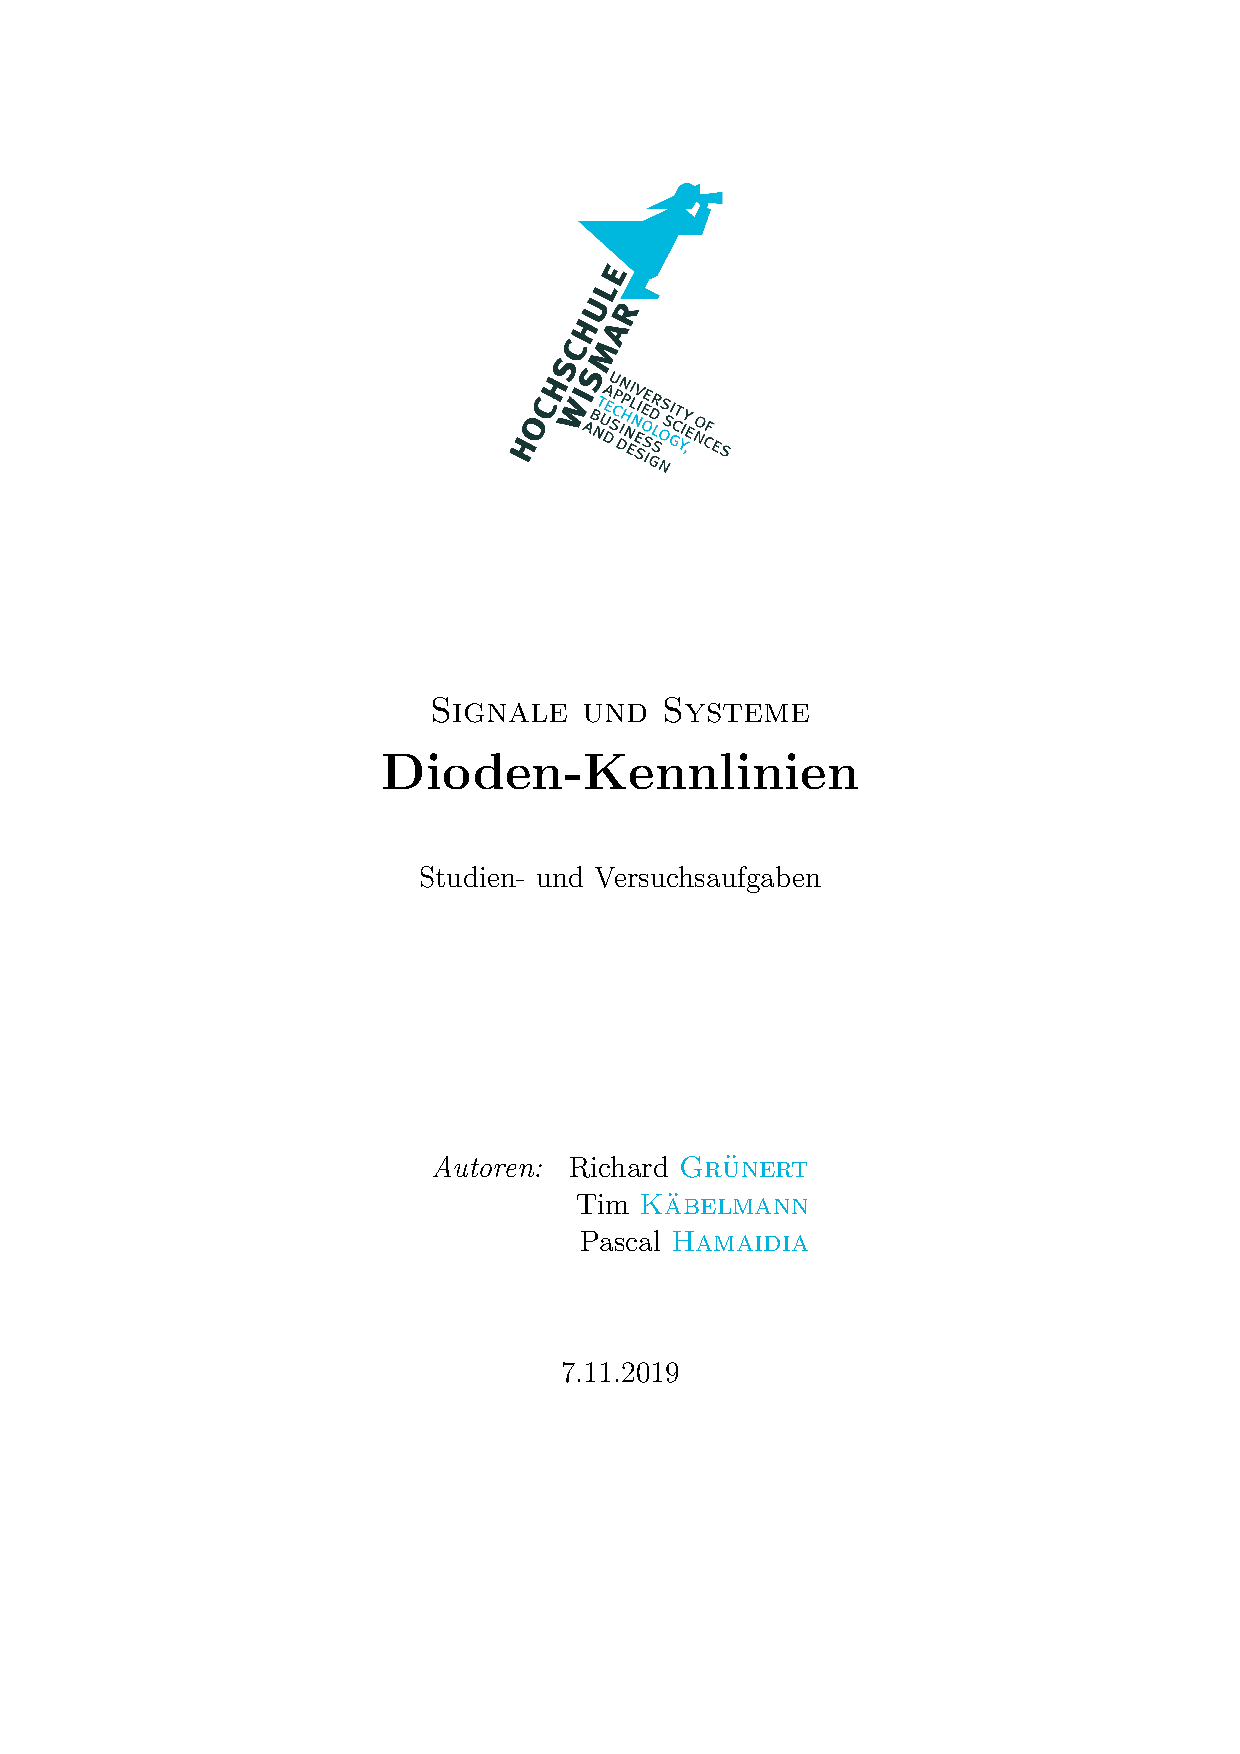
\includepdf{./titlepage/titlepage.pdf}
  \clearpage
  \setcounter{page}{1}
%%%%%%%%%%%%%%%%%%%%%%%%%%%%%%%%%%%%%

\section{Vorbereitungsaufgaben}

% 1.2
\subsection{Aufbau und Wirkungsweise eines pn-Übergangs}
\begin{center}
  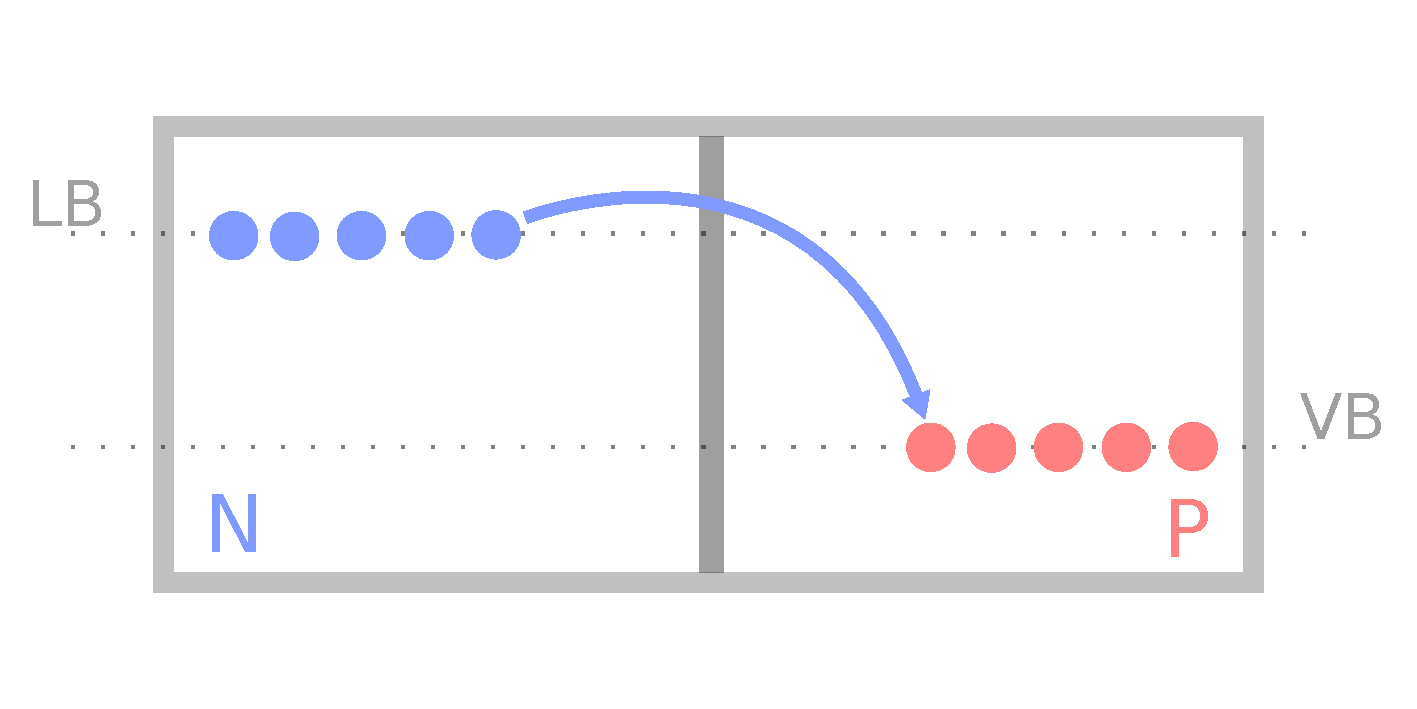
\includegraphics[width=\textwidth]{1_1/pn}
\end{center}

\noindent Dotiert man einen Halbleiterkristall (z.B. \ce{Si} oder \ce{Ge}) mit
Fremdatomen, wird die elektrische Leitfähigkeit des Halbleiters beeinflusst.

\begin{itemize}
\item{
    Bei Dotierung mit
    5-(oder höher-)wertigen Atomen (z.B. \ce{P} oder \ce{As}) geraten zusätzliche
    Elektronen in das Leitungsband des Halbleiterkristalls; es wird \emph{n-Leitung}
    provoziert
  }

\item{
    Bei Dotierung mit
    3-(oder geringer-)wertigen Atomen (z.B. \ce{B} oder \ce{Ga}) entstehen
    Elektronenfehlstellen im Valenzband des Halbleiterkristalls; es wird \emph{p-Leitung}
    provoziert.
  }
\end{itemize}

Die Elektronenkonzentration im n-Leiter ist somit höher als die im p-Leiter.
Bringt man unterschiedlich dotierte Halbleiter in Kontakt, kommt es durch
Diffusion zum Übergang von (höher-energetischen) Elektronen im Leitungsband des
n-Leiters in das (nieder-energetische) Valenzband des p-Leiters. Im p-Leiter
werden dann die Elektronenfehlstellen gefüllt und es entstehen negative Ionen;
Im n-Leiter werden durch die Elektronenwanderung Fehlstellen
von den Elektronen zurückgelassen, wodurch sich dort positive Ionen bilden. Die
Diffusion findet so lange statt, bis die Ladung bzw. das elektrische Feld der gebildeten Ionen einem weiteren
Elektronenübergang vollständig entgegenwirkt. Die verbleibende Übergangszone,
die den Ladungstransfer verhindert
wird folglich \emph{Raumladungszone} genannt. 

\begin{center}
  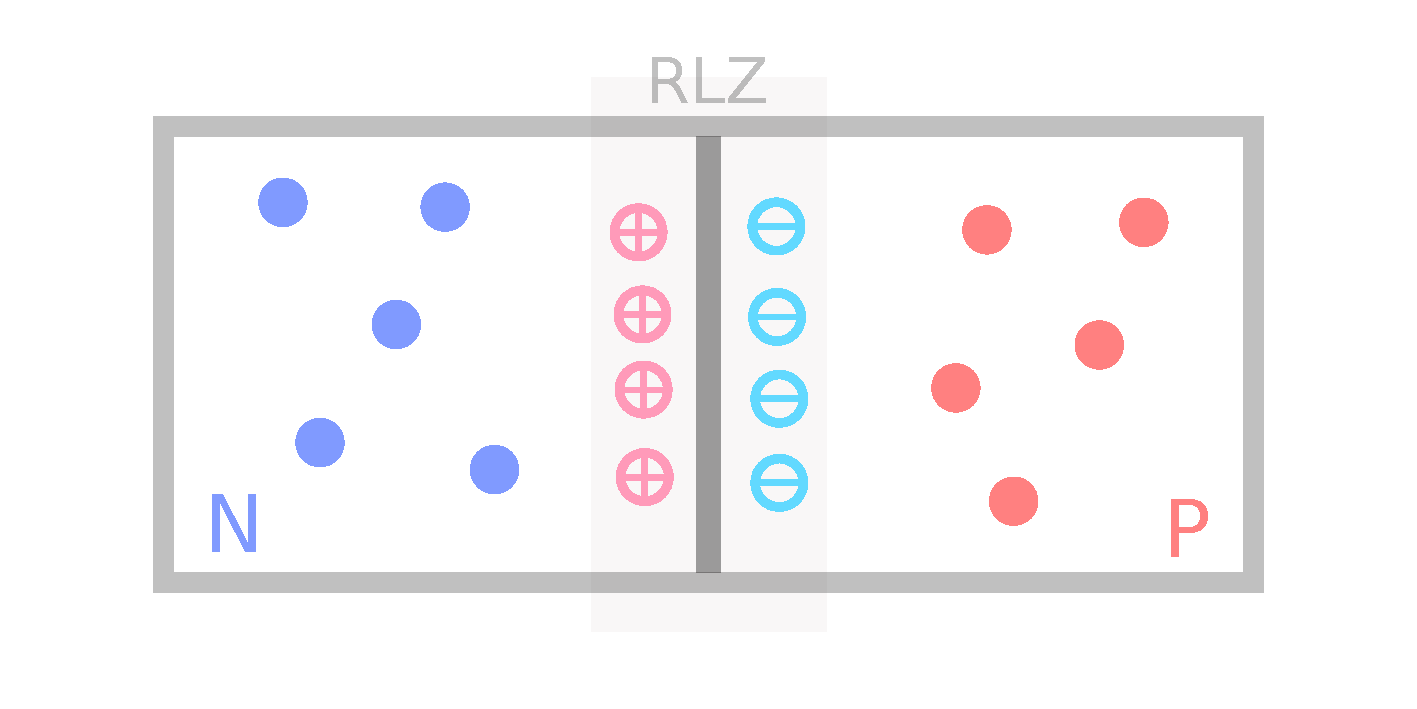
\includegraphics[width=\textwidth]{1_1/pn2}
\end{center}

% 1.1
\subsection{Aufbau und Wirkungsweise einer Diode}

\begin{center}
\begin{circuitikz}
  \draw (0,0) to[Do] (2,0);
\end{circuitikz}
\end{center}

\noindent Die elektrischen Eigenschaften des pn-Übergangs können technisch ausgenutzt werden, um eine \emph{Diode} zu realisieren. Der Stromfluss durch den pn-Übergang ist von der Polarität der über ihn angelegten Spannung abhängig. Man definiert daher die Orientierung der Diode in \emph{Sperr-} und \emph{Durchlassrichtung}.

Will man einen Strom durch die Diode treiben, so müssen die Elektronen des
n-Gebiets bzw. die Fehlstellen des p-Gebiets die Raumladungszone überqueren können.
Legt man eine negative Spannung über den pn-Übergang/die Diode, das heißt positives Potential an den n- und
negatives an den p-Leiter, wirkt die Influenz des äußeren elektrischen Feldes
so, dass sich die Majoritätsladungsträger des jeweiligen Gebiets (Elektronen im n-
und 'Fehlstellen' im p-Gebiet) von der Raumladungszone entfernen und diese somit
vergrößern\footnote[1]{Fehlstellen bewegen sich nicht tatsächlich, sondern nur modellhaft.
Sie stellen die positiv geladenen, \emph{ortsfesten} Atomrümpfe dar, die u.a. durch die
Elektronenbewegung hinterlassen werden.}. Die Diode nimmt einen statischen Zustand (bezüglich der
Majoritätsladungsträger) ein und wirkt somit elektrisch isolierend/sperrend. Reale Dioden besitzen allerdings eine
maximale Sperrspannung, ab welcher sie durchbrechen und ihre
Sperreigenschaft verlieren.


\begin{center}
  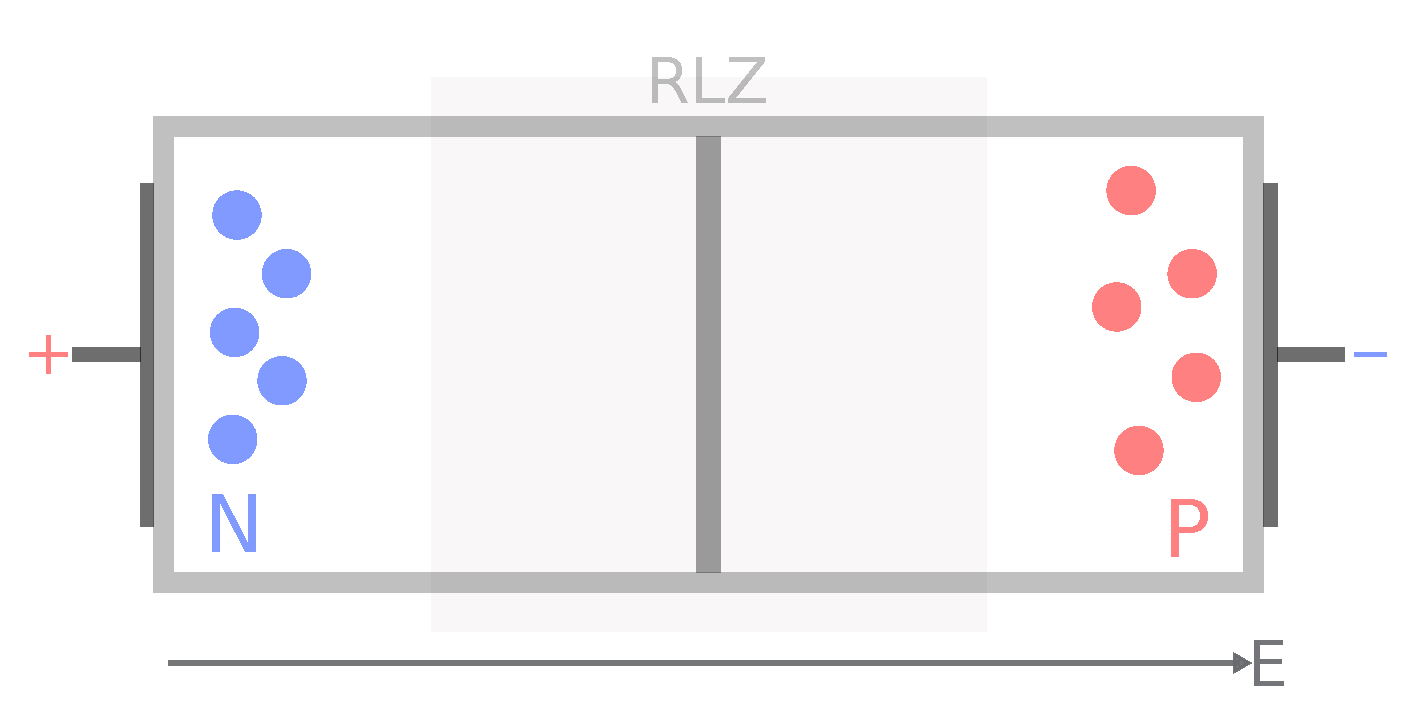
\includegraphics[width=\textwidth]{1_2/diode1}
\end{center}

Legt man eine (ausreichend) positive Spannung über die Diode, also positives Potential an den
p- und negatives an den n-Leiter, bewegen sich die Majoritätsladungsträger des
jeweiligen Bereichs in Richtung der Raumladungszone und verkleinern diese
dadurch. In dieser Richtung wirkt die Diode elektrisch leitfähig.

\begin{center}
  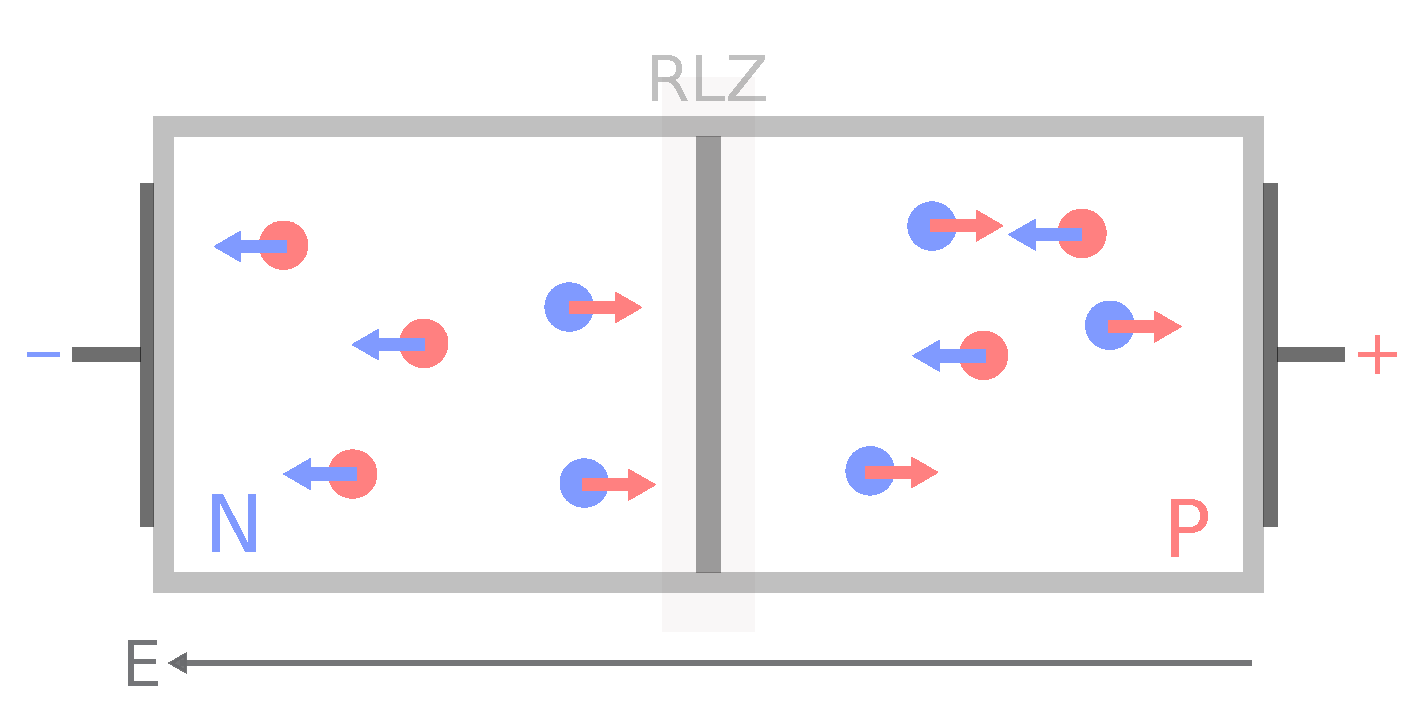
\includegraphics[width=\textwidth]{1_2/diode2}
\end{center}


% 1.3
\subsection{Z- und Schottky-Dioden}

% Z-Dioden
\begin{center}
\begin{circuitikz}
  \draw (0,0) to[Zener diode] (2,0);
\end{circuitikz}
\end{center}

Die Z-Diode ist eine besondere Diodenbauform, die kontrolliert im Durchbruchbereich
arbeiten kann. In Sperrrichtung betrieben arbeitet sie bis zu einer bestimmten
\emph{Z-Spannung}, ab welcher sie durchbricht und ihre Leitfähigkeit
exponentiell steigt. Im Durchlassbereich verhält sich die Z-Diode dagegen wie
eine normale Diode.
Z-Dioden eignen sich zur Realisierung von Spannungsstabilisierungsschaltungen (1.4).

\holine{\textwidth}

% Schottky-Dioden
\begin{center}
\begin{circuitikz}
  \draw (0,0) to[Schottky diode] (2,0);
\end{circuitikz}
\end{center}

Schottky-Dioden haben keinen üblichen Halbleiter-Halbleiter-, sondern einen Metall-Halbleiter-Übergang.
Charakteristisch sind niedrige Durchlassspanunngen im Bereich von $150 - 450 \si{\milli\volt}$.



% 1.4
\subsection{Spannungsstabilisierungsschaltung}

\begin{center}
\begin{circuitikz}
  \draw (0, 0) to[V=$U_e$] (0,-3);
  \draw (0, 0) to[R=$R_V$] (4,0);
  \draw (4,-3) to[Zener diode, *-*] (4,0);
  \draw (4,0) to[short] (6,0);
  \draw (6,0) to[R=$R_L$] (6,-3);
  \draw (0,-3) to[short] (6,-3);
\end{circuitikz}
\end{center}

% 1.5
\subsection{Dimensionierung des Vorwiderstands}

\begin{align*}
  U_{e_{\textrm{min}}} &= 8.5 \,\ \si{\volt}\\
  U_{e_{\textrm{max}}} &= 12.0 \,\ \si{\volt}\\
  I_{L_{\textrm{min}}} &= 50 \,\ \si{\milli\ampere}\\
  I_{L_{\textrm{max}}} &= 130 \,\ \si{\milli\ampere}\\
  U_{Z} &= 5.6 \,\ \si{\volt}\\
  I_{Z_{\textrm{min}}}/I_{Z_{\textrm{max}}} &= 20 \,\ \si{\milli\ampere} / 300 \,\ \si{\milli\ampere}\\
\end{align*}

\begin{gather*}
  R_{V_{\textrm{min}}} = \frac{}{}\\
  R_{V_{\textrm{max}}} = \frac{}{}
\end{gather*}

% 1.6
\subsection{Diodenkennlinie}

\begin{center}
  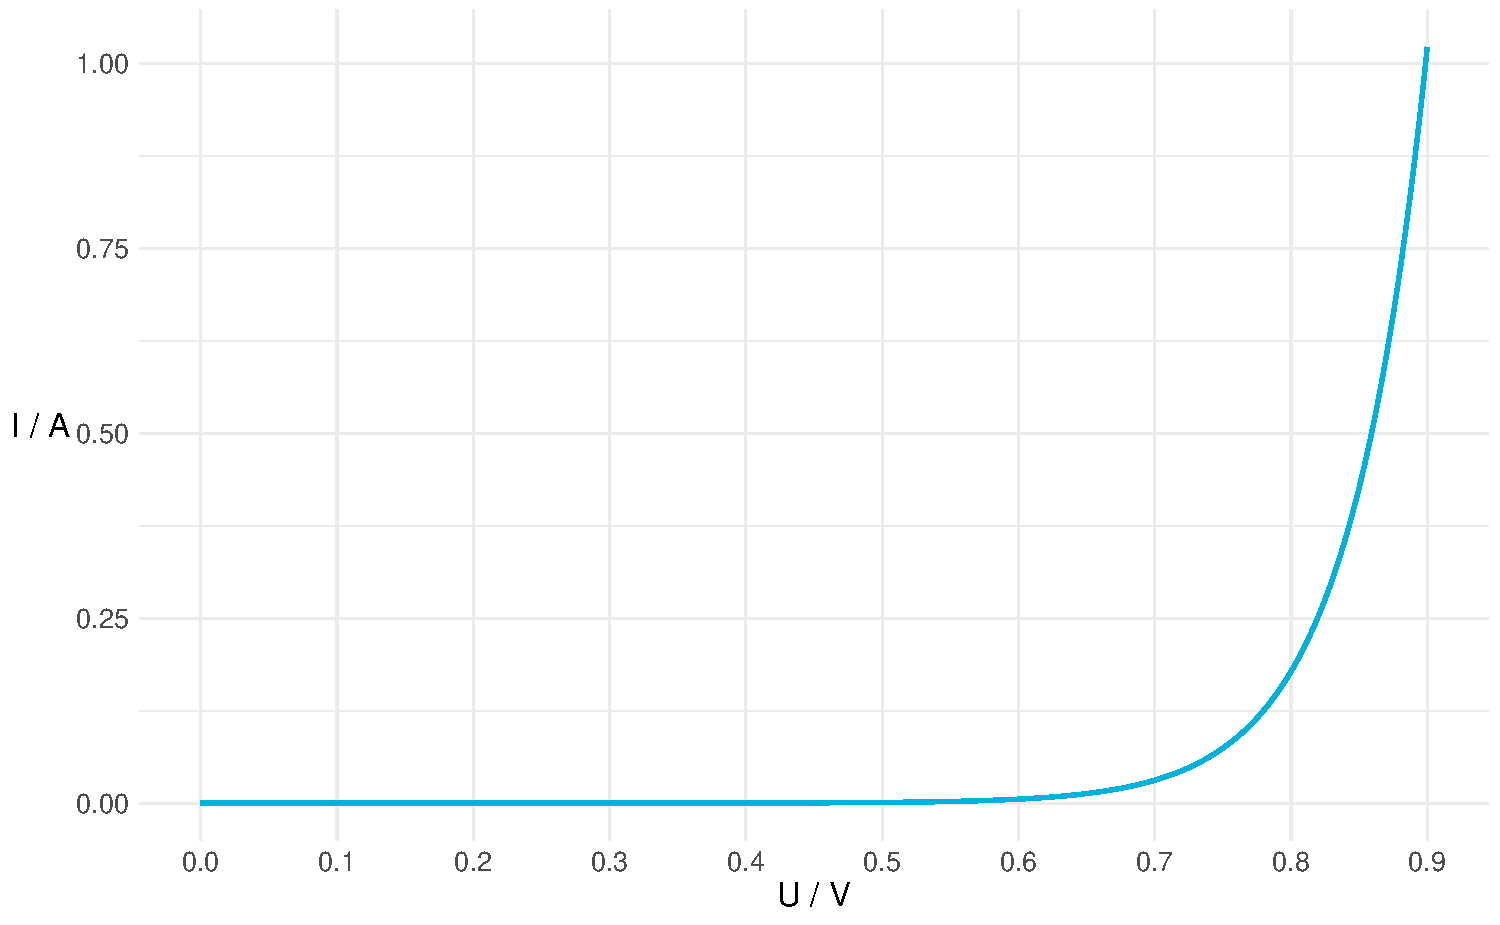
\includegraphics[width=\textwidth]{1_6/diodenkennline}
\end{center}


% 1.7
\subsection{Diodengrenzwerte}


% 2
%%%%%%%%%%%%%%%%%%%%%%%%%%%%%%%%%%%%%
\section{Versuchsaufgaben}

% 2.1
\subsection{Diodenkennline BY500}

% 2.2
\subsection{Diodenkennline ZY5,6}

% 2.3
\subsection{Z-Spannung und differentieller Widerstand}

% 2.4
\subsection{Spannungsstabilisierung bei veränderlicher Eingangsspannung}

% 2.5
\subsection{Spannungsstabilisierung bei veränderlichem Laststrom}

\end{document}
